\documentclass[border=2mm]{standalone}
\usepackage{pgfplots}
\pgfplotsset{compat=1.18}
\definecolor{red}{rgb}{0.7, 0.11, 0.11}
\definecolor{blue}{rgb}{0.0, 0.20, 0.42}
\definecolor{green}{rgb}{0.11, 0.35, 0.02}
\usepgfplotslibrary{groupplots}
\begin{document}
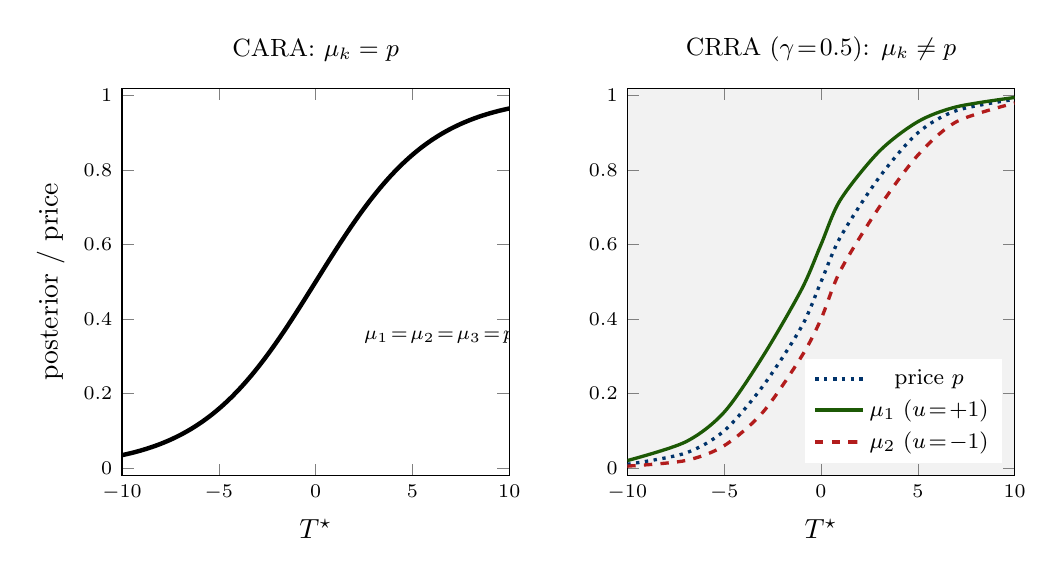
\begin{tikzpicture}
\begin{groupplot}[
  group style={group size=2 by 1, horizontal sep=15mm},
  width=6.5cm, height=6.5cm,
  xmin=-10, xmax=10, ymin=-0.02, ymax=1.02,
  xlabel={$T^{\star}$},
  title style={font=\small},
  ticklabel style={font=\scriptsize},
  legend style={draw=none,font=\footnotesize}]

% CARA panel: all posteriors = price = Lambda(T*/3)
\nextgroupplot[ylabel={posterior / price},title={CARA: $\mu_k = p$}]
\addplot[ultra thick,color=black,smooth,domain=-10:10,samples=40]
  {1/(1+exp(-x/3))};
\node[font=\scriptsize,anchor=west] at (axis cs:2,0.35) {$\mu_1\!=\!\mu_2\!=\!\mu_3\!=\!p$};

% CRRA panel: posteriors fan out
\nextgroupplot[title={CRRA ($\gamma\!=\!0.5$): $\mu_k \neq p$},
  axis background/.style={fill=black!5},
  legend pos=south east]
% Price (middle)
\addplot[very thick,color=blue,dotted,smooth] coordinates {
  (-10,0.01)(-7,0.04)(-5,0.10)(-3,0.22)(-1,0.38)(0,0.50)
  (1,0.62)(3,0.78)(5,0.90)(7,0.96)(10,0.99)};
% mu1 (u=+1, above price)
\addplot[very thick,color=green,smooth] coordinates {
  (-10,0.02)(-7,0.07)(-5,0.15)(-3,0.30)(-1,0.48)(0,0.60)
  (1,0.72)(3,0.85)(5,0.93)(7,0.97)(10,0.995)};
% mu2 (u=-1, below price)
\addplot[very thick,color=red,dashed,smooth] coordinates {
  (-10,0.005)(-7,0.02)(-5,0.06)(-3,0.15)(-1,0.30)(0,0.40)
  (1,0.53)(3,0.70)(5,0.84)(7,0.93)(10,0.98)};
\legend{price $p$, $\mu_1$ ($u\!=\!+1$), $\mu_2$ ($u\!=\!-1$)}

\end{groupplot}
\end{tikzpicture}
\end{document}
